\subsection{manually}

Why do we select a manually way to split the whole program?

\begin{itemize}
    \item It is not easy to exceed the stack depth limitation as we just put data into stack which is needed by current chunk ;
    \item It only committes data which only used in current chunk;
    \item We just need to implement gadgets to support ZKP verification as any computaion could generate a ZK proof;
    \item Executing the rust program to generate the input and output of each chunk;
    \item It keeps the lowest costs when verify the expected input and output on chain;
    \item The logic of each chunk is readable;
\end{itemize}

This approach maybe generate more chunks, but just like we said before, there will only one script chunk executed on Bitcoin. So it's acceptable.
The overall flow of manually fragment as follow pictures:
\begin{figure}[ht] 
    \centering  
    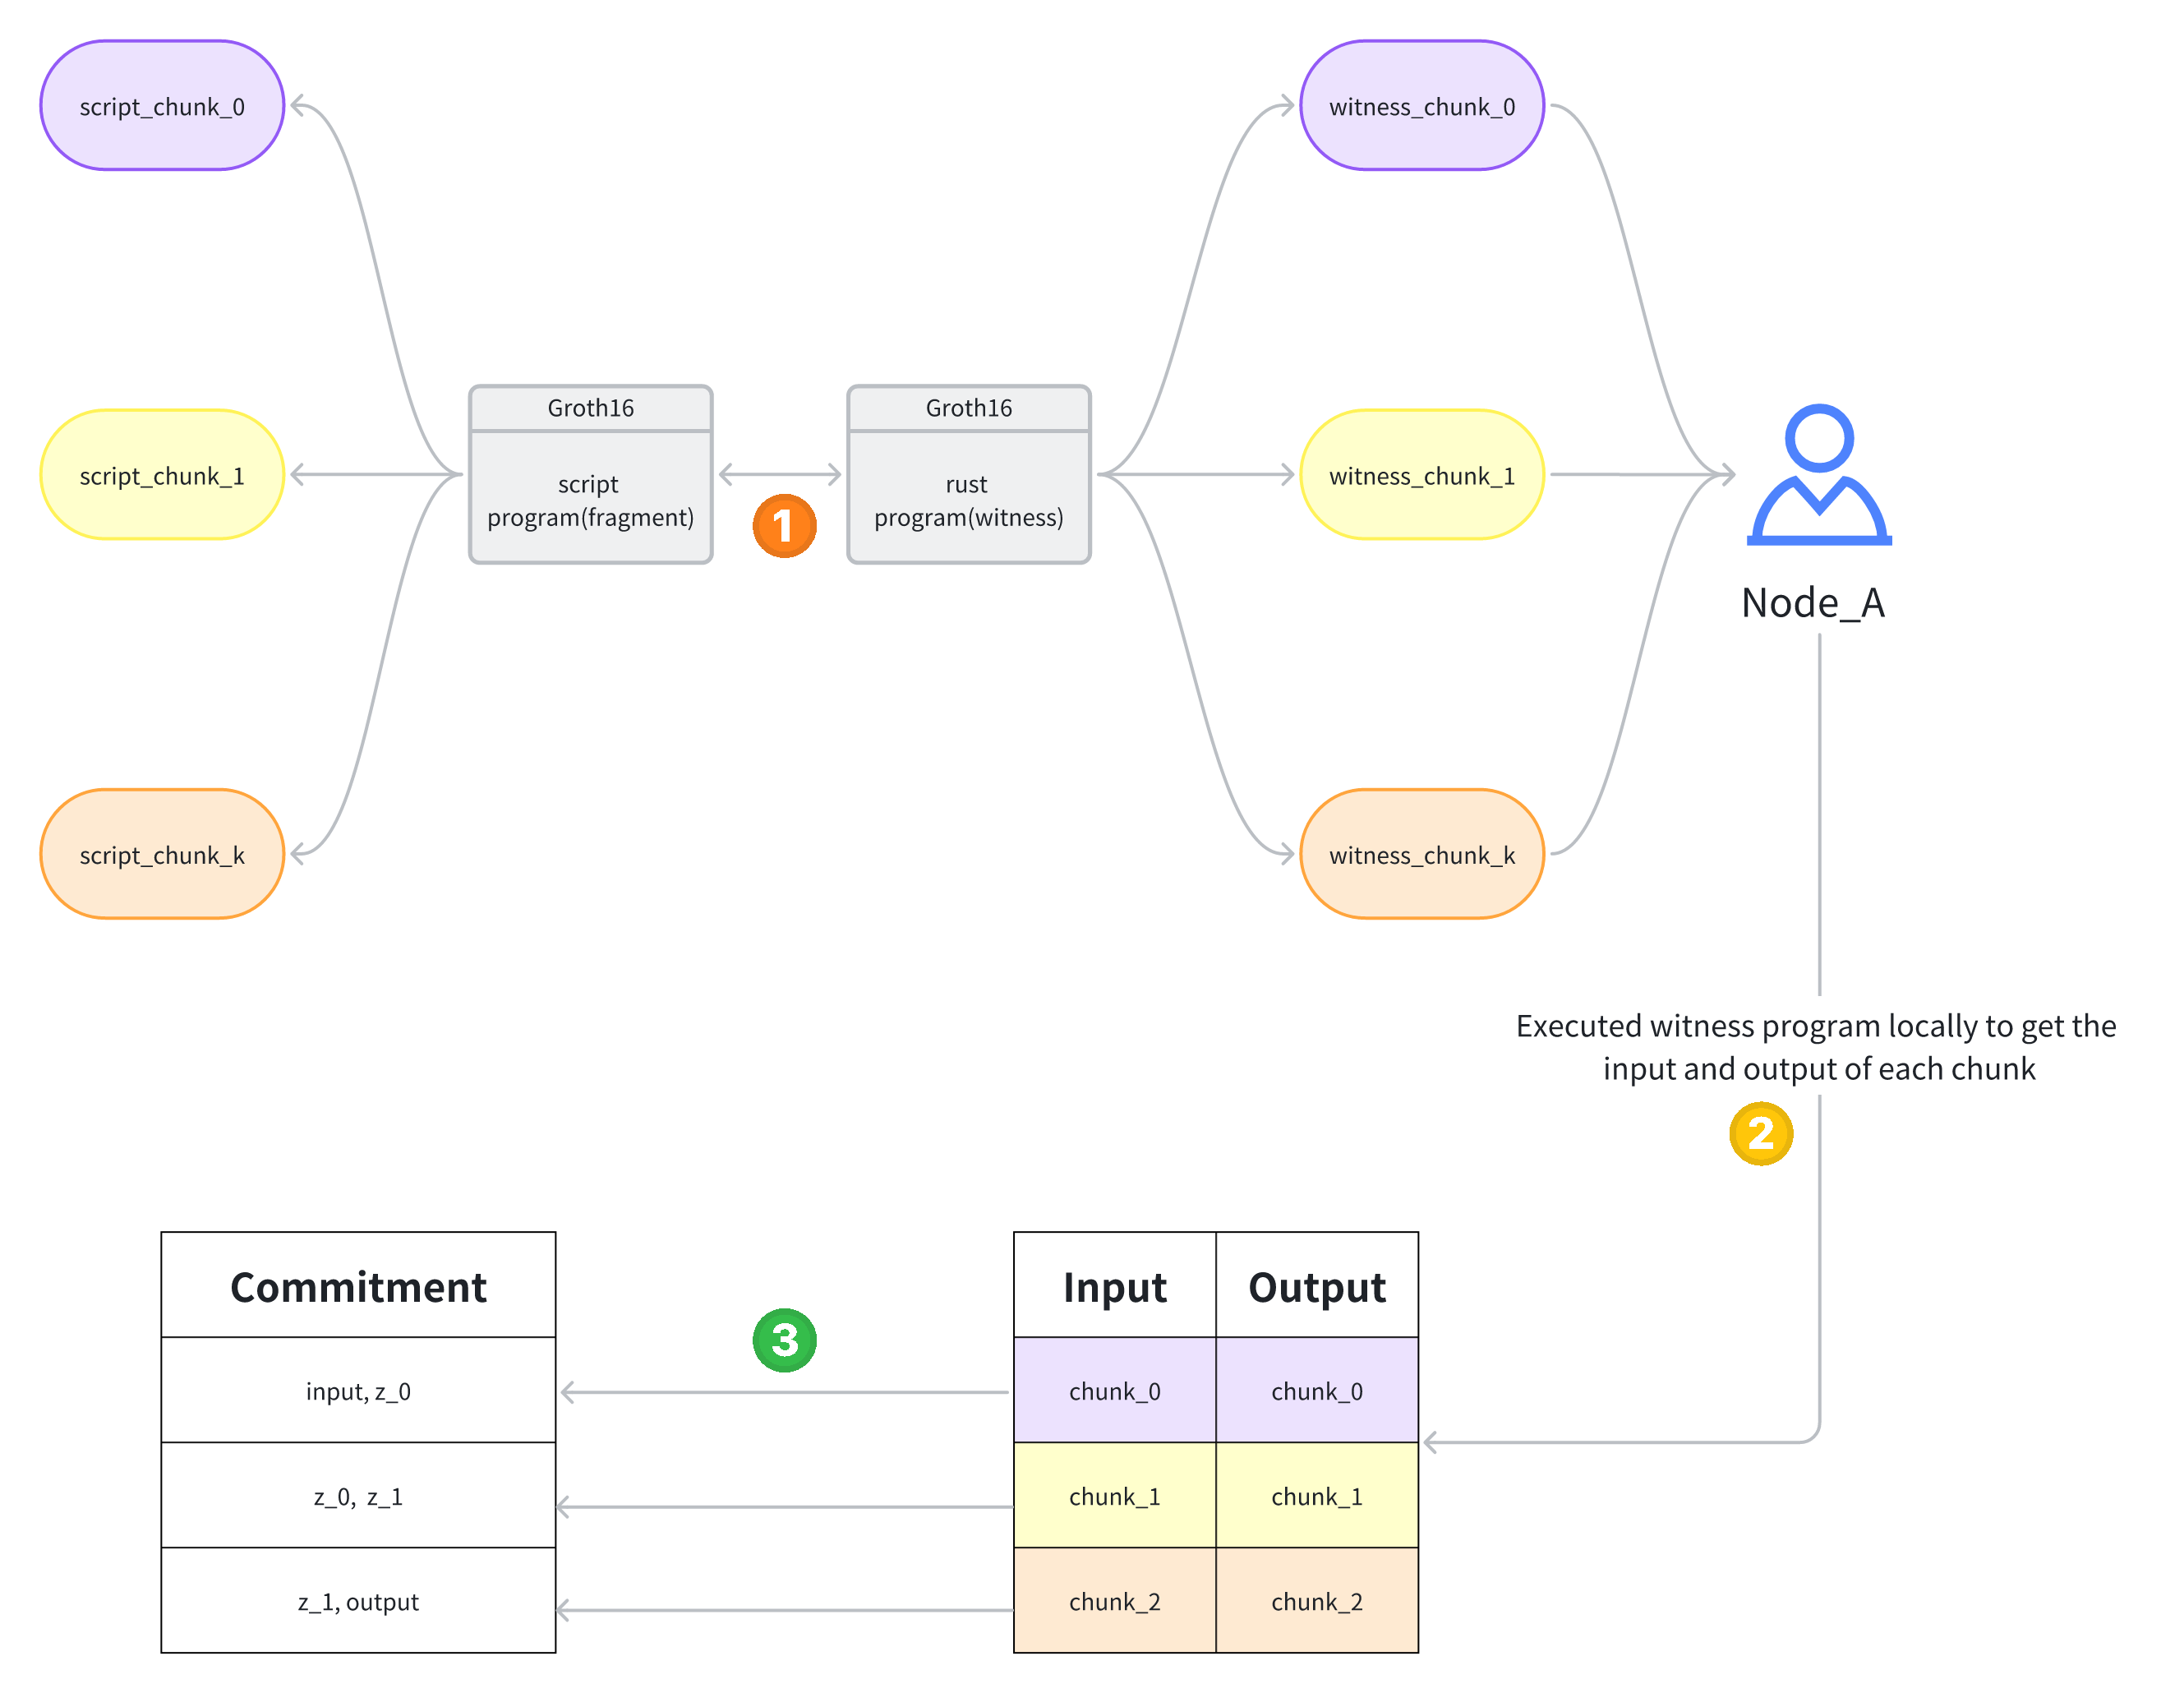
\includegraphics[width=0.85\columnwidth]{images/manually-fragment.png} 
    \caption{manually fragment}
    \label{fig:manually-fragment}
\end{figure}

The overall flow shoule be as follows:
\begin{itemize}
    \item We implememnt the rust version and script version of Groth16 ZKP verification cocurrently first;
    \item The rust verion includes the witness generation of each chunk;
    \item The script verion includes all chunks we split;
    \item We keep each chunk satisfies the size constraint and depth constraint;
    \item The Node A execute the rust program locally to generates input and output for each chunk;
    \item The Node A committes all the inputs and outputs;
\end{itemize}